\chapter{\system{}: analisi dei requisiti} \label{chap:problema} % 3

% Questo capitolo ha l'obiettivo di introdurre il problema affrontato nella tesi. Dopo una prima definizione generale, verranno analizzati in dettaglio gli input e gli output attesi dal sistema, evidenziandone le principali caratteristiche. Successivamente, saranno identificati i requisiti e i vincoli progettuali che guideranno lo sviluppo della soluzione. Il capitolo si concluderà con una rappresentazione sintetica del sistema con un diagramma di contesto.

\section{Analisi manuale delle botnet} % 3.1

All'interno dell'ambito della sicurezza informatica, la \emph{threat research} si occupa di raccogliere, analizzare e condividere informazioni (\emph{cyber threat information}) riguardanti minacce esistenti o emergenti. Tali evidenze possono essere ulteriormente elaborate fino alla produzione di \emph{threat intelligence reports} \cite{johnson2016threatintelligence}, documenti che descrivono le \emph{tactics, techniques, and procedures} (TTPs) adottate dai \emph{threat actors}, insieme alle tipologie di sistemi e di informazioni presi di mira.

% Nel caso delle botnet, la \emph{threat research} può riguardare, tra le altre attività, la caratterizzazione e il reverse engineering del protocollo di \emph{Command-and-Control} C\&C utilizzato.

Una possibile applicazione della \emph{threat research} nel contesto delle botnet consiste nella caratterizzazione e nel reverse engineering del protocollo C\&C utilizzato. La ricostruzione del protocollo può consentire di interpretare le comunicazioni tra i bot e l'infrastruttura C\&C, permettendo di identificare e analizzare i comandi trasmessi e, più in generale, di studiare il comportamento della botnet.

% Conoscenza sia nelle tecniche di analisi del malware sia nelle caratteristiche e nelle tecniche impiegate dal malware stesso.
% L'obiettivo dell'esperto di cybersecurity è quello di capire come funziona il malware in generale ma sopratutto fare il reverse engineering del protocollo C\&C.

Per svolgere tale attività, un esperto di cybersecurity, una volta entrato in possesso di un campione di malware appartenente a una botnet, può eseguirne la malware analysis, ricorrendo a tecniche di analisi statica o dinamica, combinandole tra loro e scegliendo quelle più adatte al campione. A tale scopo, l'esperto si avvale delle proprie conoscenze teoriche e della propria esperienza, integrandole, quando necessario, con le informazioni ricavate dalla consultazione di fonti e documentazione disponibili online.

% o ad altre metodologie di SRE

Quando l'esperto ha raccolto tutte le informazioni rilevanti sul protocollo C\&C, può realizzare un modulo per la cattura dei messaggi, da qui in avanti indicato come \capture{}. Il \capture{} implementa esclusivamente le funzionalità necessarie per comunicare con l'infrastruttura C\&C e simulare il comportamento di un bot, con l'obiettivo di condurre un'attività di \emph{botnet infiltration} \cite{caballero2009dispatcher}. A tal fine, il modulo si connette all'infrastruttura, presentandosi come una potenziale vittima, interagisce con essa e cattura i messaggi ricevuti. Questi possono essere successivamente salvati e utilizzati per analisi più approfondite e su scala più ampia, considerando contemporaneamente più botnet.

% insieme minimo di funzionalità

Il processo descritto è riassunto nella \Cref{fig:context_diagram_human}, che illustra sia la fase di creazione del modulo, attraverso l'analisi del campione di malware, sia quella del suo utilizzo operativo, durante la quale vengono catturati i messaggi.

% mediante un diagramma di contesto

\begin{figure}[t]
    \centering
    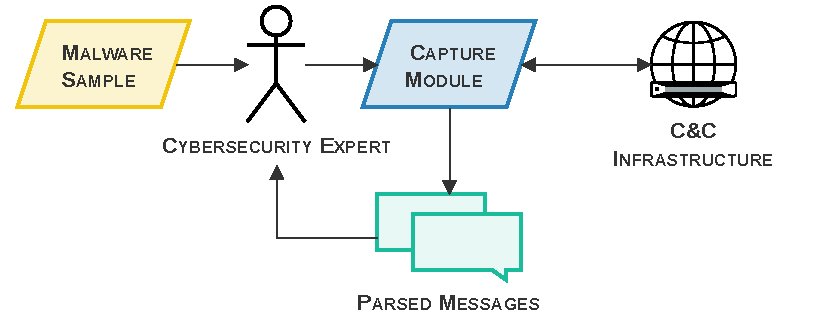
\includegraphics[width=0.95\textwidth]{img/context_diagram_human.pdf}
    \caption[Creazione e utilizzo del \capture{}]{Creazione del \capture{} da parte dell'umano e successivo utilizzo per l'infiltrazione e la cattura dei messaggi C\&C.}
    \label{fig:context_diagram_human}    
\end{figure}

% Il vantaggio di questo approccio, oltre alla possibilità per l'esperto di cybersecurity di acquisire nuove conoscenze.

Il vantaggio di questo approccio risiede soprattutto nel mantenimento del controllo diretto dell'intero processo, che permette all'esperto di distribuire tempo e risorse tra i diversi aspetti in relazione alla loro rilevanza e alla difficoltà riscontrata. Tuttavia, il lavoro manuale richiesto rimane oneroso, anche quando l'esperienza acquisita e l'adozione di pratiche volte a velocizzarlo ne migliorano l'efficienza.

Considerando che l'esperto probabilmente analizzerà botnet differenti, nella realizzazione dei \capture{} cercherà, quando possibile, di mantenere un'architettura e un comportamento uniformi, ad esempio adottando un'interfaccia comune e un formato strutturato per i messaggi catturati. Questo evidenzia ulteriormente i limiti dell'approccio manuale, che richiede un processo lungo e spesso ripetitivo, aumentando il carico cognitivo richiesto. Infine, non bisogna sottovalutare il fatto che tale processo possa richiedere competenze specialistiche di malware analysis, che non tutti i threat researcher necessariamente possiedono.

\section{\system{}} % 3.2

Un'opportunità per ridurre il carico sull'esperto di cybersecurity consiste nell'automatizzare, interamente o parzialmente, le attività di analisi del campione e la successiva creazione del \capture{}. La presente tesi si concentra proprio su questo aspetto, proponendo il sistema \system{} come soluzione al problema descritto.

% Il sistema non dovrà imporre alcun vincolo sulla natura o sul formato del file fornito e questo può in linea di principio non essere di natura malevola.

Il sistema dovrà essere progettato per ricevere in input un file binario arbitrario, di seguito indicato come \binary{}, che nella pratica operativa corrisponderà generalmente a un campione di malware in formato eseguibile appartenente a una botnet. Un ulteriore input, di natura opzionale, è rappresentato da una \kb{}, il cui utilizzo non deve costituire un prerequisito per il funzionamento di \system{}. Essa può fornire al sistema un insieme di conoscenze utili a supportare e migliorare l'attività di analisi, quali documentazione tecnica, istruzioni operative specifiche, informazioni relative a una determinata famiglia di botnet o altri contenuti ritenuti rilevanti. La natura dell'output restituito dal sistema dipenderà dall'esito della valutazione del \binary{}: qualora il file sia riconosciuto come un campione malevolo riconducibile a una botnet e sia ritenuto meritevole di analisi, il sistema dovrà svolgere tutte le attività necessarie alla costruzione del \capture{}; altrimenti, qualora vi sia certezza che non sia di interesse, il processo potrà essere interrotto e il file sarà scartato. % (risparmiando risorse)

L'obiettivo principale di \system{} consiste quindi nell'acquisire le informazioni necessarie al reverse engineering del protocollo C\&C utilizzato, al fine di sviluppare un \capture{} basato sulle proprietà specifiche della botnet in esame. Non è invece richiesta una comprensione completa delle caratteristiche e del funzionamento interno del malware analizzato, anche se ciò potrebbe essere una conseguenza collaterale dell'analisi. \system{} adotta infine un approccio \emph{best-effort}, volto a ottenere il risultato atteso attraverso le attività di analisi previste, senza tuttavia poter garantire, per ogni campione, la piena funzionalità del \capture{} prodotto, né la completezza o l'accuratezza della sua implementazione.

% , senza però rientrare tra le responsabilità del sistema -> la comprensione completa

% In questo modo, parte dei compiti precedentemente demandati all'esperto viene automatizzata, consentendo di destinare le risorse dell'esperto ad altre attività.

Il diagramma di contesto riportato in \Cref{fig:context_diagram_system} fornisce una rappresentazione ad alto livello del sistema proposto, considerato come una \emph{black-box}, e dei relativi input e output. Esso evidenzia come \system{} possa essere integrato direttamente all'interno del processo descritto nella \Cref{fig:context_diagram_human}, andando a sostituire la fase relativa alle attività di analisi e produzione del codice precedentemente affidate all'esperto di cybersecurity. L'introduzione di \system{} modifica quindi il ruolo di quest'ultimo, il cui compito non consiste più prevalentemente nello studio manuale del campione, ma si orienta maggiormente verso la revisione dei risultati prodotti dal sistema. L'esperto provvede quindi alla correzione del \capture{} generato da \system{}, potendo eventualmente anche modificarlo o estenderlo in funzione delle proprie valutazioni. Il modulo così revisionato, denominato \reviewedcapture{}, può dunque essere utilizzato dall'esperto per le medesime finalità previste nel processo originale.

%L'esperto mantiene inoltre il ruolo di utilizzatore del \capture{}, avendo pieno controllo sulle eventuali attività di correzione, modifica ed estensione del modulo e potendo decidere, sulla base delle proprie valutazioni, se e come procedere alla sua esecuzione.

\begin{figure}[t]
    \centering
    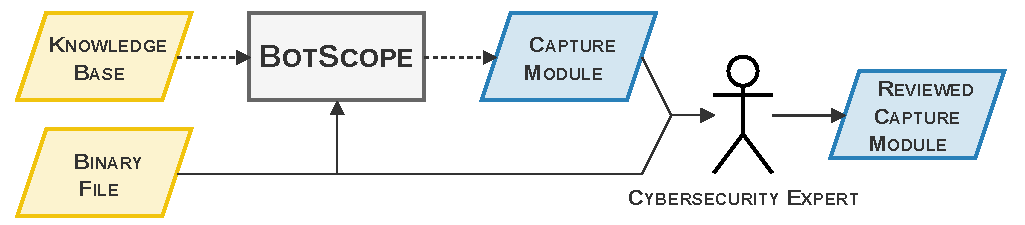
\includegraphics[width=0.95\textwidth]{img/context_diagram_system.pdf}
    \caption[Diagramma di contesto di \system{}]{Diagramma di contesto del sistema \system{}.}
    \label{fig:context_diagram_system}    
\end{figure}

% L'introduzione di \system{} modifica di conseguenza anche il ruolo dell'esperto di cybersecurity nel processo di analisi. Il suo compito non consiste più principalmente nello studio manuale del campione, ma si sposta maggiormente verso un'attività di revisione dei risultati prodotti dal sistema. L'esperto mantiene inoltre il ruolo di utilizzatore del \capture{}, avendo pieno controllo sulle eventuali attività di correzione, modifica ed estensione del modulo e potendo decidere, sulla base delle proprie valutazioni, se e come procedere alla sua esecuzione.

\subsection{Requisiti del sistema} % 3.2.1

Dopo aver definito gli obiettivi del sistema e le sue caratteristiche principali, la progettazione di \system{} non è soggetta a vincoli specifici in termini di approcci architetturali e componenti da utilizzare. Tale libertà progettuale dovrà essere esercitata nel rispetto delle metodologie e delle pratiche del \emph{software engineering}, tenendo inoltre conto dei requisiti definiti in questa fase e di quelli che emergeranno e verranno progressivamente formalizzati nel corso dello sviluppo del sistema. I quattro requisiti definiti inizialmente costituiscono i principi fondanti di \system{}, ponendone le basi architetturali, e possono essere distinti tra requisiti non funzionali e requisiti di sicurezza.

% Tale libertà progettuale dovrà tuttavia tenere conto dei requisiti definiti in questa fase e di quelli che emergeranno e verranno progressivamente formalizzati nel corso dello sviluppo del sistema.

\begin{description}
    \item[Requisiti non funzionali:] \hspace{1em}
    
    \begin{itemize}
        \item \textbf{Indipendenza dalla famiglia di botnet}: il sistema dovrà essere progettato in modo da poter essere applicato a campioni appartenenti a differenti famiglie di botnet, senza introdurre dipendenze specifiche da una particolare tipologia o dalle caratteristiche peculiari di una singola famiglia.

        % Lo stesso principio di indipendenza dovrà essere applicato anche al protocollo di comunicazione C\&C. 

        La soluzione proposta dovrà essere in grado di gestire differenti modalità di interazione tra il malware e l'infrastruttura C\&C, indipendentemente dal protocollo di comunicazione, dalle tecnologie di trasporto o dai formati dei messaggi utilizzati.

        \item \textbf{Autonomia del processo di analisi}: il sistema dovrà operare in maniera completamente autonoma, senza richiedere interventi da parte dell'utente durante la sua esecuzione e senza disporre di alcuna conoscenza preliminare sul campione analizzato. Un utente del sistema dovrà fornire il \binary{} in ingresso e si limiterà a ricevere il risultato prodotto dal sistema al termine dell'analisi. % nel caso in cui questo (\binary{}) appartenga a una botnet
        
        % Di conseguenza, al sistema non potranno essere fornite informazioni aggiuntive relative al file di ingresso, quali, ad esempio, la famiglia di appartenenza, descrizioni del comportamento o delle funzionalità del malware, oppure il protocollo di comunicazione utilizzato.

        L'utente potrà intervenire solo a processo concluso, effettuando una revisione del lavoro svolto oppure utilizzando e modificando il \capture{}. A tal fine, è fondamentale garantire un adeguato livello di trasparenza sulle operazioni svolte dal sistema durante l'analisi, così da facilitare le attività successive svolte dall'utente.

        % L'utente potrà poi intervenire solo a processo concluso, eseguendo il modulo generato o operando su di esso, apportando correzioni o miglioramenti. A tal fine, è fondamentale garantire un adeguato livello di trasparenza rispetto alle operazioni svolte dal sistema durante l'analisi, così da agevolare la comprensione del processo da parte dell'utente e facilitare eventuali modifiche al modulo generato.

    \end{itemize}

    \item[Requisiti di sicurezza:] \hspace{1em}
    
    \begin{itemize}
        \item \textbf{Natura difensiva del modulo generato}: il \capture{} dovrà avere esclusivamente finalità difensive e dovrà limitarsi a catturare passivamente le comunicazioni C\&C. Le funzionalità implementate dovranno essere circoscritte alla gestione della connessione e alle fasi di ricezione, decodifica, classificazione e parsing dei messaggi ricevuti. Non dovranno essere inclusi comportamenti offensivi, né meccanismi volti a eseguire attacchi o altre azioni malevole. Le uniche comunicazioni attive consentite saranno quelle strettamente necessarie all'instaurazione e al mantenimento della sessione con l'infrastruttura C\&C.
        
        \item \textbf{Sicurezza del processo di analisi}: il processo di analisi del \binary{} dovrà essere progettato in modo tale da garantire la protezione dell'ambiente di esecuzione. L'elaborazione dei campioni malevoli non dovrà in alcun modo esporre il sistema di analisi, né eventuali sistemi esterni coinvolti, a rischi di compromissione o alterazione del loro funzionamento.
    \end{itemize}

\end{description}

% Oltre ai requisiti precedentemente individuati, la progettazione dell'architettura dovrà seguire i principi dell'ingegneria del software, preferendo soluzioni che garantiscano la qualità, la manutenibilità e l'estensibilità del sistema. Pur non essendo requisiti funzionali, queste proprietà condizioneranno le scelte di progettazione e implementazione.

\subsection{Proprietà del \capture{}} % 3.2.2

Al fine di favorire una semplice integrazione del sistema all'interno di workflow esterni già esistenti e pipeline di automazione più ampie, è necessario che ogni \capture{} sia conforme a un insieme di proprietà prestabilite. Tali vincoli sono stati pertanto identificati e definiti durante l'analisi dei requisiti, anticipandone la formalizzazione rispetto alle successive fasi di progettazione e implementazione.

Si è deciso quindi di fissare un linguaggio di programmazione per i \capture{}, al fine di garantire l'uniformità dei moduli, scegliendo a questo proposito Python, in virtù di due motivi principali. Il primo è l'ampio utilizzo del linguaggio nell'ambito della cybersecurity e della \emph{Network Forensics} \cite{oconnor2012python}, grazie alla disponibilità di un vasto ecosistema di librerie e strumenti dedicati all'analisi e all'elaborazione dei dati di rete. Il secondo riguarda la disponibilità di costrutti avanzati, come i generatori \cite{ramalho2022yield}, che consentono di elaborare progressivamente i messaggi C\&C secondo un modello \emph{lazy}, permettendo così di gestire il flusso di messaggi in modo efficiente anche durante l'analisi del traffico di rete in tempo reale.

% \cite{oconnor2012python} \cite{ramalho2022yield} Chapter 17

% Il primo riguarda il fatto che tale linguaggio è ampiamente utilizzato nell'ambito della cybersecurity e della \emph{Network Forensics}, grazie alla disponibilità di un ampio ecosistema di librerie e strumenti dedicati all'analisi e all'elaborazione dei dati di rete \cite{oconnor2012python}. Il secondo aspetto riguarda un requisito tecnico legato alla gestione del traffico di rete in tempo reale. L'impiego di costrutti avanzati di Python, come i generatori, attraverso l'istruzione \texttt{yield}, consente di elaborare progressivamente i messaggi C\&C secondo un modello \emph{lazy}, anziché mantenerne l'intero contenuto in memoria \cite{ramalho2022yield}. Tale approccio permette infatti di limitare il consumo di memoria del modulo, facilitandone l'integrazione con altri sistemi e rendendolo idoneo a operare per periodi di tempo prolungati. % Chapter 17

Ciascun \capture{} dovrà inoltre essere \emph{self-contained}, ovvero completamente autoconsistente, includendo al suo interno tutte le definizioni, le classi e le dipendenze necessarie a implementare in autonomia le funzionalità previste dal modulo, tra cui l'infiltrazione, la cattura del traffico, l'elaborazione e il parsing dei comandi. Infine, per favorire l'integrazione dei \capture{} all'interno di sistemi esterni e consentire la gestione scalabile di più moduli, sono stati definiti un'interfaccia standardizzata per il modulo e uno schema comune per i messaggi.

L'interfaccia del modulo, \interface{}, definisce il contratto comune a tutti i \capture{}, che ogni modulo dovrà implementare. La standardizzazione dell'interfaccia consente a qualsiasi componente che conosca tale contratto di caricare e utilizzare direttamente il modulo, senza doverne conoscere la struttura e i dettagli interni. La \interface{} stabilisce in particolare la presenza di due metodi fondamentali, \texttt{connect} e \texttt{sniff}.

Il metodo \texttt{connect} ha lo scopo di inizializzare o, eventualmente, di ripristinare la connessione con l'infrastruttura C\&C. Il metodo è progettato per essere eseguito all'avvio del \capture{}, prima dell'inizio dell'attività di cattura, e successivamente ogni volta che il metodo \texttt{sniff} terminerà la propria esecuzione a causa della chiusura della connessione o di un errore non recuperabile. Il metodo \texttt{sniff} ha lo scopo di mantenere attiva la connessione con l'infrastruttura C\&C ed eseguire la cattura passiva dei messaggi. Il metodo è progettato per rimanere in esecuzione indefinitamente e dovrà essere implementato come un generatore Python, restituendo mediante l'istruzione \texttt{yield} gli oggetti corrispondenti ai messaggi catturati, dopo averli ricevuti e decodificati.

La definizione completa della \interface{} è riportata in \Cref{fig:botnet_interface}, mentre la \Cref{fig:botnet_main} mostra un possibile utilizzo pratico di un \capture{}, la cui classe principale, \botnet{}, implementa la \interface{} definita.

\begin{figure}[t]
    \centering

    \begin{minipage}{0.45\textwidth}
        \centering
        \begin{lstlisting}[frame=single, style=pystyle]
from abc import ABC, abstractmethod
class BotnetInterface(ABC):
  @abstractmethod
  def connect(self):
    pass
  @abstractmethod
  def sniff(self):
    pass
        \end{lstlisting}
        \captionof{figure}[Definizione iniziale dell'interfaccia astratta \interface{}]{
            Definizione iniziale dell'interfaccia astratta \interface{}. \\ \hspace{1em}
        }
        \label{fig:botnet_interface}
    \end{minipage}%
    \hspace{0.05\textwidth}%
    \begin{minipage}{0.45\textwidth}
        \centering
        \begin{lstlisting}[frame=single, style=pystyle]
b = Botnet()

while True:
  try:
    b.connect()
    for message in b.sniff():
      print(message)
  except:
    pass
        \end{lstlisting}
        \captionof{figure}[Esempio di uso di un generico \capture{}]{
            Esempio di uso di un generico \capture{}, con classe principale \botnet{} che implementa \interface{}.
        }
        \label{fig:botnet_main}
    \end{minipage}%
\end{figure}

Lo schema dei messaggi, \schema{}, definisce il formato comune a cui dovranno essere conformi gli oggetti restituiti dal metodo \texttt{sniff} del \capture{}. Considerata la natura eterogenea delle botnet analizzate, caratterizzate da protocolli di comunicazione e formati dei messaggi differenti, è essenziale avere una rappresentazione uniforme dei messaggi che consenta ai componenti successivi di elaborarli indipendentemente dalla botnet di provenienza. A differenza della \interface{}, per la quale sono già stati specificati i metodi e il comportamento atteso, in questa fase non è necessario imporre vincoli sulla struttura interna del \schema{}. L'unico requisito è l'esistenza di uno schema fisso e condiviso, che potrà essere definito direttamente durante l'implementazione del sistema.